\documentclass[10pt,journal,compsoc]{IEEEtran}

% *** CITATION PACKAGES ***
%
\ifCLASSOPTIONcompsoc
  % IEEE Computer Society needs nocompress option
  % requires cite.sty v4.0 or later (November 2003)
  \usepackage[nocompress]{cite}
\else
  % normal IEEE
  \usepackage{cite}
\fi

\usepackage{graphicx}
\graphicspath{ {Images/} }
\usepackage{amssymb}
\usepackage{amsmath}
\usepackage{listings}
\usepackage{color}
\usepackage[table,xcdraw]{xcolor}

\definecolor{dkgreen}{rgb}{0,0.6,0}
\definecolor{gray}{rgb}{0.5,0.5,0.5}
\definecolor{mauve}{rgb}{0.58,0,0.82}

\lstset{frame=tb,
  language=Python,
  aboveskip=3mm,
  belowskip=3mm,
  showstringspaces=false,
  columns=flexible,
  basicstyle={\small\ttfamily}, 
  numbers=none,
  numberstyle=\tiny\color{gray},
  keywordstyle=\color{blue},
  commentstyle=\color{dkgreen},
  stringstyle=\color{mauve},
  breaklines=true,
  breakatwhitespace=true,
  tabsize=3,
  morekeywords={if, in, or, then, enter, into, end, command, delete, from, not, create},
  xleftmargin=\dimexpr 1em+3pt\relax,
  linewidth=\dimexpr \linewidth-3pt\relax
}

\lstnewenvironment{itemlisting}[1][] 
 {%
  \mbox{}
  \vspace*{-\baselineskip}
  \lstset{
    xleftmargin=\leftmargin,
    linewidth=\linewidth,
    #1 
  }%
 }
 {}
 
% correct bad hyphenation here
\hyphenation{op-tical net-works semi-conduc-tor}

\renewcommand{\arraystretch}{1.5}

\begin{document}

\title{CS 6600 Project Report: Unmanned Aircraft System}

\author{Matthew Whitesides and Bruce M. McMillin \\
Department of Computer Science \\
Missouri University of Science and Technology, Rolla, MO 65409-0350} 

% The paper headers
\markboth{Missouri S\&T COMP\_SCI 6600: Formal Methods in CmpSec, Fall~2021}%
{Shell \MakeLowercase{\textit{et al.}}: Bare Demo of IEEEtran.cls for Computer Society Journals}
 
% The paper abstract
\IEEEtitleabstractindextext{%
\begin{abstract}
The abstract goes here.
\end{abstract}}

% make the title area
\maketitle

\IEEEpeerreviewmaketitle

%-------------------------------------------------------------------------

\section{Infrastructure}

\subsection{Infrastructure Description}

\IEEEPARstart{I}{n} its simplest form, an unmanned aircraft system (UAS), is an aircraft system that operates without an onboard pilot. 
UAS are either controlled remotely through some form of wireless radio communication, semi-autonomously in conjunction with a remote pilot, or fully autonomously using some form of computational intelligence as navigation. 
These intelligent crewless vehicles have many potential uses in the defense sector, including surveillance, strategic mission execution, aerial sustainability support, and training systems, to name a few. 
These aircraft fall under the umbrella of cyber-physical systems (CPS), merging the intelligent navigation processes, system health monitoring, and communication with the physical mobile aerial vehicle.

We will design a proposed infrastructure security policy for the Boeing MQ-25 unmanned aircraft system, but it will also apply to similar mission support drones. 
The MQ-25 is an unmanned aircraft system designed for the U.S. Navy, and it provides autonomous refueling capability for the Boeing F/A-18 Super Hornet, Boeing EA-18G Growler, and Lockheed Martin F-35C fighters.
This capability extends the combat range of the supported aircraft, seamlessly and semi-anonymously navigating to the plane, refueling, and returning to base. 
MQ-25 is the first unmanned aircraft to support aerial refueling another aircraft and is currently in the flight test phase of development [1], making it the perfect system to analyze security impacts for current and future unmanned aircraft systems. For the purposes of this document we will take the basic idea of the MQ-25 and model a UAS system referred to as the MX-01 UAS. 

\subsubsection{Infrastructure Security Policy}

\begin{table}[]
  \caption{Description of rights over objects in the UAS.}
  \begin{tabular}{ll}
  \hline
  \textbf{Right}       & \textbf{Description}                               \\ 
  \hline
  \textit{Owns (O)}    & The owner of the given object.                     \\
  \textit{Read (R)}    & Can observe the given object.                      \\
  \textit{Write (W)}   & Can modify the given object.                       \\
  \textit{Execute (E)} & Can execute the functionality of the given object. \\
  \textit{Grant (G)}   & Can grant a given right to another subject.        \\
  \textit{Control (C)} & Can control a given system object.                 \\
  \textit{Delete (C)}  & Can delete a given object or right.                 \\
  \textit{Create (C)}  & Can create a new subject or object.                 \\
  \end{tabular}
\end{table}

\begin{table*}[]
  \caption{Description of actor subject roles during a UAS refueling mission.}
  \begin{tabular}{ll}
  \hline
  \textbf{Subject}                           & \textbf{Description}                                                                                       \\ 
  \hline
  \textit{Pilot Commander (PC)}                  & The primary remote pilot of the UAS during the mission.                                                    \\
  \textit{Instructor Pilot (IP)}                 & Assists the Pilot Commander and can pilot the UAS if given permission from the PC or MC.                   \\
  \textit{Maintenance Crew (MC)}                 & Handles work orders created by the PC, IP, or FDA, responsible for the maintenance of the UAS.             \\
  \textit{Flight Data Admin (FDA)}               & Handles and analyses all mission flight data.                                                              \\
  \textit{External Contractor (Bad Actor) (EC)}  & Has a similar job to the MC however only has read rights to the FED.                                       \\
  \end{tabular}
\end{table*}

\begin{table*}[]
  \centering
  \caption{Initial UAS Refueling Mission Access Control Matrix}
  \label{tab:initial-acm}
  \resizebox{\textwidth}{!}{
    \begin{tabular}{l|llllllllll}
      \hline
      \textbf{}                                        & \textit{PC}   & \textit{IP}   & \textit{MC}   & \textit{FDA}  & \textit{EC}   & \textbf{ANC}  & \textbf{RO}   & \textbf{FED}  & \textbf{RTD}  & \textbf{FRS}  \\
      \hline
      \textit{Pilot Commander (PC)}                    & O,R,W         & R,W           & R,W           & R,W           & R,W           & O,R,W,E,G,C   & O,R,W,E,G,C   & R,W,E,G,C     & R,W,E,G,C     & R,W,E,G,C     \\
      \textit{Instructor Pilot (IP)}                   & R             & O,R,W         & $\varnothing$ & $\varnothing$ & $\varnothing$ & R,W,E,C       & R,W,E,C       & R,E           & R,E           & R,E           \\
      \textit{Maintenance Crew (MC)}                   & $\varnothing$ & $\varnothing$ & O,R,W         & $\varnothing$             & R             & $\varnothing$ & $\varnothing$ & R,E           & R,E           & R,E           \\
      \textit{Flight Data Admin (FDA)}                 & $\varnothing$ & $\varnothing$ & R             & O,R,W         & O,R,W         & $\varnothing$ & $\varnothing$ & O,R,W,E,G,C   & O,R,W,E,G,C   & O,R,W,E,G,C   \\
      \textit{External Contractor (Bad Actor) (EC)} & $\varnothing$ & $\varnothing$ & $\varnothing$ & $\varnothing$ & O,R,W         & $\varnothing$ & $\varnothing$ & $\varnothing$ & R             & $\varnothing$ \\
      \textbf{Autonomous Navigation Control (ANC)}     & $\varnothing$ & $\varnothing$ & $\varnothing$ & $\varnothing$ & $\varnothing$ & R,W,E,C       & R             & R             & R             & $\varnothing$ \\
      \textbf{Refueling Operation (RO)}                & $\varnothing$ & $\varnothing$ & $\varnothing$ & $\varnothing$ & $\varnothing$ & $\varnothing$ & R,W,E,C       & R             & R             & $\varnothing$ \\
      \textbf{Flight Engine Data (FED)}                & $\varnothing$ & $\varnothing$ & $\varnothing$ & $\varnothing$ & $\varnothing$ & $\varnothing$ & $\varnothing$ & R,W,E,C       & $\varnothing$ & $\varnothing$ \\
      \textbf{Refueling Tank Data (RTD)}               & $\varnothing$ & $\varnothing$ & $\varnothing$ & $\varnothing$ & $\varnothing$ & $\varnothing$ & $\varnothing$ & $\varnothing$ & R,W,E,C       & $\varnothing$ \\
      \textbf{Flight Record System (FRS)}              & $\varnothing$ & $\varnothing$ & $\varnothing$ & $\varnothing$ & $\varnothing$ & $\varnothing$ & $\varnothing$ & $\varnothing$ & $\varnothing$ & R,W,E,C      
    \end{tabular}}
  \end{table*}

  \begin{table*}[]
    \centering
    \caption{ACM After Create Flight Record}
    \label{tab:table-after-create-flight-record}
    \resizebox{\textwidth}{!}{
    \begin{tabular}{l|lllllllllll}
      \hline
      \textbf{}    & \textit{PC}                          & \textit{IP}                          & \textit{MC}                          & \textit{FDA}                         & \textit{EC}                          & \textbf{ANC}                         & \textbf{RO}                          & \textbf{FED}                         & \textbf{RTD}                         & \textbf{FRS}                         & {\color[HTML]{009901} \textbf{FR}}   \\
      \hline
      \textit{PC}  & O,R,W                                & R,W                                  & R,W                                  & R,W                                  & R,W                                  & O,R,W,E,G,C                          & O,R,W,E,G,C                          & R,W,E,G,C                            & R,W,E,G,C                            & R,W,E,G,C                            & {\color[HTML]{009901} R,W,E,G,C}     \\
      \textit{IP}  & R                                    & O,R,W                                & $\varnothing$                        & $\varnothing$                        & $\varnothing$                        & R,W,E,C                              & R,W,E,C                              & R,E                                  & R,E                                  & R,E                                  & {\color[HTML]{009901} R,E}           \\
      \textit{MC}  & $\varnothing$                        & $\varnothing$                        & O,R,W                                & $\varnothing$                                    & R                                    & $\varnothing$                        & $\varnothing$                        & R,E                                  & R,E                                  & R,E                                  & {\color[HTML]{009901} R,E}           \\
      \textit{FDA} & $\varnothing$                        & $\varnothing$                        & R                                    & O,R,W                                & O,R,W                                & $\varnothing$                        & $\varnothing$                        & O,R,W,E,G,C                          & O,R,W,E,G,C                          & O,R,W,E,G,C                          & {\color[HTML]{009901} O,R,W,E,G,C}   \\
      \textit{EC}  & $\varnothing$                        & $\varnothing$                        & $\varnothing$                        & $\varnothing$                        & O,R,W                                & $\varnothing$                        & $\varnothing$                        & $\varnothing$                        & R                                    & {\color[HTML]{CB0000} E,W}             & {\color[HTML]{009901} $\varnothing$} \\
      \textbf{ANC} & $\varnothing$                        & $\varnothing$                        & $\varnothing$                        & $\varnothing$                        & $\varnothing$                        & R,W,E,C                              & R                                    & R                                    & R                                    & $\varnothing$                        & {\color[HTML]{009901} $\varnothing$} \\
      \textbf{RO}  & $\varnothing$                        & $\varnothing$                        & $\varnothing$                        & $\varnothing$                        & $\varnothing$                        & $\varnothing$                        & R,W,E,C                              & R                                    & R                                    & $\varnothing$                        & {\color[HTML]{009901} $\varnothing$} \\
      \textbf{FED} & $\varnothing$                        & $\varnothing$                        & $\varnothing$                        & $\varnothing$                        & $\varnothing$                        & $\varnothing$                        & $\varnothing$                        & R,W,E,C                              & $\varnothing$                        & $\varnothing$                        & {\color[HTML]{009901} $\varnothing$} \\
      \textbf{RTD} & $\varnothing$                        & $\varnothing$                        & $\varnothing$                        & $\varnothing$                        & $\varnothing$                        & $\varnothing$                        & $\varnothing$                        & $\varnothing$                        & R,W,E,C                              & $\varnothing$                        & {\color[HTML]{009901} $\varnothing$} \\
      \textbf{FRS} & $\varnothing$                        & $\varnothing$                        & $\varnothing$                        & $\varnothing$                        & $\varnothing$                        & $\varnothing$                        & $\varnothing$                        & $\varnothing$                        & $\varnothing$                        & R,W,E,C                              & {\color[HTML]{009901} $\varnothing$} \\
      {\color[HTML]{009901} \textit{\textbf{FR}}} & {\color[HTML]{009901} $\varnothing$} & {\color[HTML]{009901} $\varnothing$} & {\color[HTML]{009901} $\varnothing$} & {\color[HTML]{009901} $\varnothing$} & {\color[HTML]{009901} $\varnothing$} & {\color[HTML]{009901} $\varnothing$} & {\color[HTML]{009901} $\varnothing$} & {\color[HTML]{009901} $\varnothing$} & {\color[HTML]{009901} $\varnothing$} & {\color[HTML]{009901} $\varnothing$} & {\color[HTML]{009901} R,W,E,C}      
    \end{tabular}}
  \end{table*}

  Our infrastructure security policy breaks down the various actions a system user can perform using the following terms. 

  \begin{itemize}
    \item \textit{Subject}: Any entity that contains the proper rights can request the UAS perform operations, access objects, or grant rights to another subject.
    \item \textit{Object}: An entity that is part of the UAS functionality or data that does not have control over another entity. 
    \item \textit{Rights}: A property assigned to a subject that defines its right to access an object or grant permissions to another subject.
  \end{itemize}
  
  Table 1 describes the rights and their associated functionality. Table 2 breaks down the subject roles involved in operating the UAS during a refueling mission. Table 3 contains the access control matrix (ACM) showing each Subject's rights over the objects.
  
  \subsection{HRU}

  The Harrison, Ruzzo, Ullman security model (HRU) establishes a finite set of mono-operational procedures our system can perform on subjects and objects. Given our set of rights and ACM, we will establish a set of commands available to the system that acts upon the subjects and objects in the system. The commands will consist of mono-operational modifications and pre-condition checks. Therefore given these sets, we can show how a specific set of commands can create a rights leakage. 
  
  The following shows the basic HRU commands related to our UAS mission.
  A fundamental UAS refueling mission follows these basic steps. 

  \begin{enumerate}
    \item UAS is verified flight-ready by the MC.
    \item The PC plans the mission.
    \item The PC and IP execute the mission.
    \item During the flight, the PC and IP execute the ANC and RO as needed.
    \item After the refueling operation, the UAS returns to base, and the flight is debriefed. 
    \item PC, IP, or MC download the flight data from the UAS flight recorder. 
    \item A flight record (FR) is created that contains flight tracking information, engine usage data, and various UAS health status.
    \item This flight record is uploaded by the PC, IP, MC, or EC to the record-keeping system. 
    \item Mission is completed. 
  \end{enumerate}
  
  With this in mind, we have the following basic HRU commands available for post-flight maintenance (steps 5 - 9). We will then show how improper use of these commands can lead to a rights leakage with our external contractor standing in as our ``bad actor'' gaining a leak of Integrity and confidentiality rights beyond our initial ACM. 

  The first command is a generic \textit{Grant r Rights} that allows a subject to grant any right they have over a subject/object to another subject/object.

\begin{lstlisting}
command grant_r_right(r, o, p, q)
  if grant in A[p, o] and r in A[p, o]
  then
    enter r into A[q, o];
end
\end{lstlisting}
    
  Next we have command \textit{Make Owner} allowing a subject \textit{p} to make another subject \textit{q} the owner of a object \textit{o} they currently have owner rights over. 

\begin{lstlisting}
command make_owner(p, q, o)
  if owns in A[p, o]
  then
    enter owns into A[q, o];
end
\end{lstlisting}
  
  When the \textit{PC} and \textit{IP} return from a flight they or a \textit{MC} will read the flight data and create a new object \textbf{Flight Record (FR)} holding the flight data, available to subjects who have \textbf{FED} access. 
  After running this command, our ACM would transition to a new state similar to Table 4, representing the subjects and objects involved in the create flight record procedure. 
  This command will also give rights to the FRS to control the flight record data once uploaded.
  
\begin{lstlisting}
command create_flight_record(p)
  if create in A[p, FED]
  then
    create object FR;
    enter own into A[p, FR];
    enter delete into A[p, FR];
    enter read into A[p, FR];
    enter grant into A[p, FR];
end
\end{lstlisting}

After creating a flight record which may be done by a PC, IP, or MC, they may choose to give the task of processing and uploading the flight record to an external external contractor and execute the following command to provide them with access to the record. 
In the command \textit{Grant Flight Record Access}, \textit{p} is the subject granting the right to subject \textit{q}, for the \textit{fr} flight record.

\begin{lstlisting}
command grant_flight_record_access(p, q, fr)
if own in A[p, fr]
then
  enter read into A[q, FR];
  enter write into A[q, FR];
  enter execute into A[q, FR];
end
\end{lstlisting}  

Finally, the flight record needs to be uploaded to our flight record system using the following \textit{Upload Flight Record} command with \textit{p} being the subject executing the command and \textit{fr} being flight record to upload.

\begin{lstlisting}
command upload_flight_record(p, fr)
if own in A[p, fr] and read in A[p, FRS]
then
  enter read into A[FRS, FR];
  enter write into A[FRS, FR];
  enter execute into A[FRS, FR];
  enter control into A[FRS, FR];
end
\end{lstlisting}

Similar to \textit{Create Flight Record} a subject may need to delete or update a flight record from the system. 

\begin{lstlisting}
command delete_flight_record_from_system(p, FR)
if delete in A[p, FR]
then
  delete read from A[FRS, FR];
  delete write from A[FRS, FR];
  delete execute from A[FRS, FR];
  delete control from A[FRS, FR];
end
\end{lstlisting}

If any modifications need to be made to the FRS, the following command begins an update transaction and ends one for a given subject and flight record. 

\begin{lstlisting}
command update_flight_record_system(p, FR)
if own in A[p, FR]
  then
    enter read into A[p, FED];
    enter read into A[p, FR];
    enter write into A[p, FED];
    enter write into A[p, FR];
  end
\end{lstlisting}

\subsection{Rights Leakages}
  
\subsubsection{Confidentiality}

  For our example of a confidentiality attack, we simulate a scenario where our \textit{External Contractor} is a bad actor seeking leaked rights beyond the initial ACM utilizing the following HRU commands available for the UAS.

  The following sequence of commands is typical among a mission debriefing process. 

\begin{lstlisting}
create_flight_record(Maintenance Crew (MC));
grant_flight_record_access(Maintenance Crew, External Contractor (EC), Flight Record (FR));
upload_flight_record(External Contractor (EC), Flight Record (FR));
\end{lstlisting}  

  However, when running \textit{upload\_flight\_record}, the EC will find they do not have ``own'' rights over the record, which is required so that they will go back to the original MC and as to grant them execute privileges to the FRS system. 
  The MC will execute the commands to make EC have permission to upload the FR. 

\begin{lstlisting}
make_owner(MC, EC, FR);
command grant_r_right(execute, FRS, MC, EC);
\end{lstlisting}

  This command, unfortunately, will lead to a leak as the contractor (EC) now has the execute privileges over the FRS, which they did not initially and is not intended and can lead to other flight records confidential information being exposed to the EC. 
  Table 4 shows the leaked rights in red. 

\subsubsection{Integrity}

  In an attempt at an integrity leak, our EC may seek to modify existing data and, to get permission to do so, may attempt the following sequence. 

\begin{lstlisting}
create_flight_record(Maintenance Crew (MC));
upload_flight_record(External Contractor (EC), Flight Record (FR));
grant_flight_record_access(Maintenance Crew, External Contractor (EC), Flight Record (FR));
make_owner(MC, EC, FR);
update_flight_record_system(EC, FR);
\end{lstlisting}  

  However, upon reviewing the FR, the MC notices an issue in the data and wants the EC to update the flight record system. 
  Unfortunately, \textit{Update Flight Record System} checks only for rights to the given flight record and not the initial systems, therefore, giving the EC \textit{write} access to the FRS system, which could lead them modifying the FRS data ruining its integrity.
  Table 4 shows the result of executing the confidentiality and integrity leaks. 

\section{Survey}

\subsection{Take-Grant}

Next, we take a look at the Take-Grant (TG) model interpretation of our rights leakages. 
This model represents our system as a directed graph, with our subject and objects represented as vertices (black for subjects, white for objects). 
Edges represent the rights on vertex has over another, where special take (\textit{t}) and grant (\textit{g}) representing the ability of a subject or object to give or obtain rights from another subject or object. 
In our case, subjects can execute a grant HRU command representing the grant right, and take can be achieved by rights automatically allocated by granting access to specific objects (i.e., the FRS).

This models our HRU example in terms of a TG model where the \textit{Flight Record} created object has \textit{read, write} rights over the \textit{Flight Record System} that our \textbf{External Contractor (EC)} can utilize to gain \textit{read, write} access to the \textit{Flight Engine Data}.

Our bad actor could achieve this leak through the following TG commands. 

\begin{enumerate}
  \item \textbf{MC} creates object \textbf{FR}.
  \item \textbf{MC} grants (\textit{t} to \textbf{FR}) to \textbf{EC}.
  \item \textbf{EC} takes (\textit{r,w} to \textbf{FRS}) from \textbf{FR}.
  \item \textbf{EC} takes (\textit{r,w} to \textbf{FED}) from \textbf{FRS}.
\end{enumerate}

Figure 1 shows the initial state of rights among actors and objects in the \textbf{FRS} system.

\begin{figure}[t]
  \caption{Initial Iteration T-G Model Graph} 
  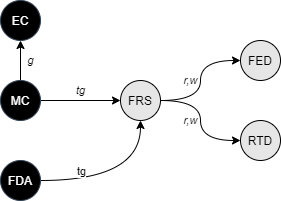
\includegraphics[scale=0.7]{TGModel1.png}
\end{figure}

Figure 2 shows the state of rights after the \textbf{MC} runs the HRU command \textit{create\_flight\_record(MC)} which a new \textbf{FR} object. 

\begin{figure}[t]
  \caption{Iteration 2 T-G Model Graph} 
  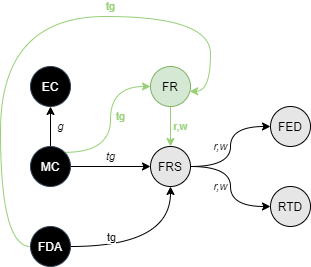
\includegraphics[scale=0.7]{TGModel2.png}
\end{figure}

Figure 3 shows the state after the \textbf{EC} leads the \textbf{MC} into giving them \textit{t} rights over \textbf{FR} they can exploit the system to take our leaked rights to \textbf{FED} through the \textbf{FRS}. 
This would be established after the command \textit{grant\_flight\_record\_access(MC, EC, FR)}.

\begin{figure}[t]
  \caption{Iteration 3 T-G Model Graph} 
  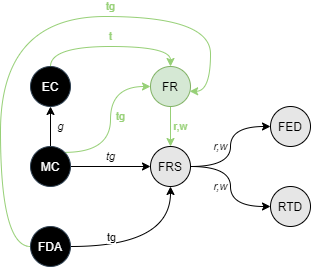
\includegraphics[scale=0.7]{TGModel3.png}
\end{figure}

Therefore allowing EC to execute \textit{update\_flight\_record\_system(EC, FR)} which leaks access to the FED as shown by the state in Figure 4.

\begin{figure}[t]
  \caption{Final Iteration T-G Model Graph} 
  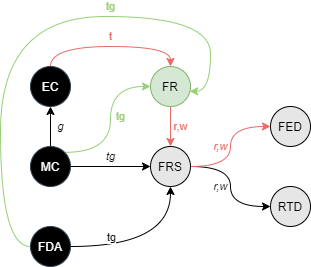
\includegraphics[scale=0.7]{TGModel4.png}
\end{figure}

Using this TG protection model instead of the simple HRU commands, we demonstrate that the safety question is decidable in linear time based on our graph consisting of seven nodes.

\subsection{Bell-LaPadula}
The Bell-LaPadula Model (BLP) focuses on establishing access control confidentiality through security levels and categories. 
BLP focuses on two simple rules in a security policy within a given ACM. 
The simple security property states a subject can not read an object at a higher security level. 
The star property states that a subject may not write to any object at a lower security level.

The primary limitation we see when implementing a BLP model into our existing policy is our external contractor and maintenance controllers. We need access to the flight records, so they require at least \textit{confidential} clearance levels. These restrictions make it hard to read the flight record system at a \textit{secrete} level and our FRS to write to the flight records. 

For our BLP implementation, we first define the security classifications for our subjects and objects. Given we are dealing with military records, it makes sense to use the standard government security levels. In addition to the security level, subjects and objects will fall into categories based upon the appropriate work unit.  
Table 5 shows the security clearance levels and the subjects/objects at the given levels.
Table 6 shows the work unit categories of each subject/object.

\begin{table}[]
  \caption{Security Classifications for the UAS}
  \label{tab:security-classifications}
  \centering
  \begin{tabular}{lll}
  \hline
  \textbf{Clearance Level} & \textbf{Subjects} & \textbf{Objects} \\
  \hline
  Top Secret (TS)          & PC, FDA           & ANC, RO          \\
  Secret (S)               & IP                & FRS, RTD         \\
  Confidential (C)         & MC, EC            & FED, FR          \\
  Unclassified (UC)        &                   &                 
  \end{tabular}
\end{table}

\begin{table}[]
  \caption{Work Unit Categories for the UAS}
  \label{tab:work-unit-categories}
  \centering
  \begin{tabular}{lll}
  \hline
  \textbf{Category}        & \textbf{Subjects} & \textbf{Objects} \\
  \hline
  Flight Ops (FO)          & PC,IP         & ANC,RO          \\
  Maintenance Ops (MO)     & PC,IP,MC,FDA  & FED,RTD,FR,FRS    \\
  Flight Data Ops (FDO)    & PC,IP,FDA,EC  & FED,FR,FRS             
  \end{tabular}
\end{table}

Now that we've established security classifications for our subjects and objects, we can see how the system and security policy could still allow leakage and further theft of flight record data. 

\begin{lstlisting}
  create_flight_record(Maintenance Crew (MC));
  grant_flight_record_access(Maintenance Crew, External Contractor (EC), Flight Record (FR));
  upload_flight_record(External Contractor (EC), Flight Record (FR));
  make_owner(MC, EC, FR);
  update_flight_record_system(EC, FR);
\end{lstlisting}  

\begin{enumerate}
  \item \textbf{MC} executes \textit{create flight record} creating flight record object \textbf{FR}.
  \begin{itemize}
    \item This write is allowed as the object \textbf{FR} created has clearance level of \textit{Confidential} which is greater than or equal to \textbf{MC's} level of \textit{Confidential} and \textbf{FR} dominates \textbf{MC} by categories.
  \end{itemize}
  \item \textbf{MC} executes \textit{upload flight record} granting the object \textbf{FRS} access to the flight record object \textbf{FR}.
  \begin{itemize}
    \item This write is allowed as the object \textbf{FRS} created has clearance level of \textit{Secret} which is greater than \textbf{FR's} level of \textit{Confidential} and \textbf{FRS} dominates \textbf{MC} by categories.
  \end{itemize}
  \item \textbf{MC} executes \textit{grant flight record access} granting \textbf{EC} access flight record object \textbf{FR}.
  \begin{itemize}
    \item This read is allowed as the subject \textbf{EC} created has clearance level of \textit{Confidential} which is greater than or equal to \textbf{FR's} level of \textit{Confidential} and \textbf{MC} dominates \textbf{EC} by categories.
  \end{itemize}
  \item \textbf{MC} executes \textit{make owner} making \textbf{EC} have owner rights over flight record object \textbf{FR}.
  \begin{itemize}
    \item This write is allowed as the subject \textbf{EC} created has clearance level of \textit{Confidential} which is greater than or equal to \textbf{FR's} level of \textit{Confidential} and \textbf{FR} dominates \textbf{EC} by categories.
  \end{itemize}
  \item \textbf{EC} executes \textit{update flight record system} allowing \textbf{EC} write to the flight record system object \textbf{FRS}.
  \begin{itemize}
    \item This write is allowed as the subject \textbf{EC} created has clearance level of \textit{Confidential} which is less than or equal to \textbf{FRS's} level of \textit{Secret} and \textbf{FRS} dominates \textbf{EC} by categories.
  \end{itemize}
\end{enumerate}

As you can see, while this system does keep our bad actor \textbf{EC} from reading the confidential flight records from the flight record system, it does not prevent an integrity attack of writing up to the \textbf{FRS} and \textbf{FR}.

We can setup our BLP system state in the context of the command leakages as follows:

\begin{itemize}
  \item $S = \{MC, EC\}$
  \item $O = \{FRS, FR\}$
  \item $P = \{owner, read, write\}$
  \item $C = \{Secret (S), Confidential (C)\}$
  \item $K = \{MO, FDO\}$
  \item $f_c(s) = \{(C, \{MO\}), (C, \{FDO\})\}$
  \item $f_c(o) = \{(S, \{MO, FDO\}), (C, \{MO, FDO\})\}$
\end{itemize}

Then as the commands are executed we can see the resulting states in Table 7. 

\begin{table*}[]
  \centering
  \caption{BLP System State Commands}
  \label{tab:blp-commands}
    \begin{tabular}{llllll}
      \hline
      \textbf{} & \textbf{$i_0$}                                      & \textbf{$i_1$}                & \textbf{$i_2$}        & \textbf{$i_3$}        & \textbf{$i_4$}        \\
      \hline
      X         & \{(r, $\varnothing$), ($\varnothing$, $\varnothing$)\} & \{(r, $\varnothing$), (r, o)\} & \{($\varnothing$, r), ($\varnothing$, $\varnothing$)\} & \{($\varnothing$, o), ($\varnothing$, $\varnothing$)\} & \{($\varnothing$, w), ($\varnothing$, $\varnothing$)\} \\
      Y         & \{(y, n), (n, n)\}                                  & \{(y, n), (y, y)\}            & \{(y, y), ($\varnothing$, y)\}   & \{(y, y), ($\varnothing$, y)\}   & \{($\varnothing$, y), (y, y)\}   \\
      Z         & $V_1$                                               & $V_2$                         & $V_3$                 & $V_4$                 & $V_5$                
      \end{tabular}
  \end{table*}

\subsection{Biba}

The Biba model focuses on data integrity as opposed to the BLP model, which enforces confidentiality by restricting access. The Biba model ensures the data objects once created remain unmodified by untrusted sources by establishing integrity levels. 
The model achieves this by ensuring ACM transitions do not allow subjects to write/modify data above their integrity level. Subjects do not read data below their level to avoid being influenced by data below their trusted level. 

These notions apply to our infrastructure well as the bad actor (External Contractor), in theory, could either read data they're not supposed to (violating confidentiality). Or the EC could modify existing flight record data (violating integrity). If the confidentiality policy is perfectly implemented, no data is accessed that is outside their security level. However, there's still an amount of "trust" we have in the EC and system preventing the integrity of the data from being violated. The Biba model attempts to quantify this level of trust and maintain the flow of information, inhibiting its modification by lower trusted subjects/objects. 

\subsection{BLP-Biba Lipner Like}

Lipner proposed an integrity model that combined aspects of the BLP and Biba model to fit a more real-world commercial software development environment. Lipner created security levels and categories similar to BLP to prevent various software development lifecycle subjects from accessing different systems. Lipner then added to the security classifications with integrity classifications for system programs and integrity categories to differentiate development and production environments. 

In our BLP model we established various security classifications (Table 5) and work unit categories (Table 6) so we need to establish security categories to define the area of impact in the given category (Table 8).

We can now incorporate integrity categories to allow distinction between on aircraft systems and the flight record keeping system (Table 9) and integrity classifications to determine the trust of the data combing from that source (Table 10 highest to lowest level).  

This gives us an overall security and integrity clearance levels for subject categories (Table 11) and objects (Table 12). 

Ideally, these classifications would block EC from accessing FRS by putting them in a lower classification stopping our rights leakage. However, due to the requirement of MC to allow EC to read a flight record, our system would not operate otherwise. 


\begin{table}[]
  \caption{Security Categories for the UAS}
  \label{tab:security-categories}
  \centering
  \begin{tabular}{lll}
  \hline
  \textbf{Security Category} & \textbf{Subjects} & \textbf{Objects} \\
  \hline
  Archived Data (AD)         & PC,MC,FDA         & FRS              \\
  Operational Data (OD)      & PC,IP,MC          & ANC,RO,FED,RTD   \\
  Ready To Load (RTL)        & FDA,MC,EC         & FR,FRS    
  \end{tabular}
\end{table}

\begin{table}[]
  \caption{Integrity Categories for the UAS}
  \label{tab:integrity-categories}
  \centering
  \begin{tabular}{lll}
  \hline
  \textbf{Integrity Category} & \textbf{Subjects} & \textbf{Objects}  \\
  \hline
  On Aircraft (IOA)            & PC,IP,MC        & ANC,RO,FED,RTD \\
  Flight Record System (IFRS)  & FDA,MC,EV       & FRS        
  \end{tabular}
\end{table}

\begin{table}[]
  \caption{Integrity Classifications for the UAS}
  \label{tab:integrity-classifications}
  \centering
  \begin{tabular}{lll}
  \hline
  \textbf{Integrity Classifications} & \textbf{Subjects} & \textbf{Objects} \\
  \hline
  System Programs (ISP)                  & $\varnothing$    & ANC,RO,FRS     \\
  Operational (IO)                       & PC,IP,FDA        & $\varnothing$  \\
  Maintenance (IM)                       & MC,EC            & FRS,FED,RTD,FR      
  \end{tabular}
\end{table}

\begin{table}[]
  \caption{Security and Integrity Levels for Work Units}
  \label{tab:security-integrity-work-units}
  \centering
  \begin{tabular}{lll}
  \hline
  \textbf{Work Unit Category} & \textbf{Security} & \textbf{Integrity} \\
  \hline
  Flight Ops                  & (\{TS,\{OD\})    & (ISP,\{IOA\})      \\
  Maintenance Ops             & (\{S,\{AD,RTL\}) & (IO,\{IOA,IFRS\})  \\
  Flight Data Ops             & (\{S,\{OD,RTL\}) & (IM,\{IFRS\})      
  \end{tabular}
\end{table}

\begin{table}[]
  \caption{Security and Integrity Levels for Objects}
  \label{tab:security-integrity-objects}
  \centering
  \begin{tabular}{lll}
  \hline
  \textbf{Object} & \textbf{Security} & \textbf{Integrity}   \\
  \hline
  ANC             & (\{TS,\{OD\})       & (ISP,\{IOA\})      \\
  RO              & (\{TS,\{OD\})       & (ISP,\{IOA\})      \\
  FED             & (\{S,\{AD,OD,RTL\}) & (IO,\{IOA,IFRS\})  \\ 
  RTD             & (\{S,\{OD\})        & (IO,\{IOA,IFRS\})  \\
  FRS             & (\{S,\{AD,OD,RTL\}) & (IM,\{IFRS\})  
  \end{tabular}
\end{table}

\begin{figure}[t]
  \caption{Aircraft Systems COI Class} 
  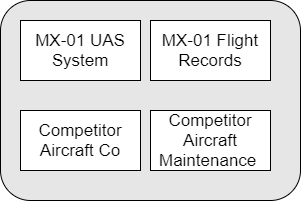
\includegraphics[scale=0.5]{COI_Classes.png}
\end{figure}

\subsection{Clark Wilson}

The Clark Wilson is an integrity verification model that enforces a principle of \textit{separation of duty} in that a subject/object that verifies a data state transition is not the same one that caused it. Data with valid integrity is defined to be in a \textit{consistant state}, and processes can only transform data through valid \textit{transactions} that preserve this consistency. Data that is constrained by the separation of duty and transaction controls are said to be \textit{constrained data items (CDIs)}. In contrast, data not constrained by these are called \textit{unconstrained data items (UDIs)}. 

After defining out CDIs, we define two procedures, an \textit{integrity verification procedure (IVP)} that tests the system is in a valid state, and \textit{transformation procedures (TPs)} that will change the state of the system using transactions. To ensure valid TPs occur on valid CDIs, the Clark Wilson model has various \textit{certification rules (CR)} that ensures the TPs and IVPs that operate on CDIs keep a valid state and \textit{enforcement rules {ER}} that prevent TPs from operating on CDIs that have not been certified.

First, for our scenario, we'll define the CDIs and UDIs. In this, we'll describe the contained data items as data related to the flight record and the unconstrained being the autonomous operations. While on their own, the ANC and RO are vital, and access should be confidential. The integrity check, in this case, is specific to the flight record data. 

\begin{itemize}
  \item $CDIs=\{FED, RTD, FRS, FR\}$
  \item $UDIs=\{ANC, RO\}$
\end{itemize}

Next, we need to establish the \textit{integrity constraints} over the flight record data. 

\begin{itemize}
  \item The FRs uploaded to the FRS must be equivalent to the data on the UAS as it is transferred over to the FRS.
  \item The FRS can only be written via new FRs or deleted, but FRs themselves cannot change.
\end{itemize}

Next, we will define the IVP commands that run on the system to ensure these constraints have been adhered to. 
After an executed upload, the first IVP check rereads the FR from the UAS and compares it to the FR in the FRS.
The next IVP ensures that the FRS is not modified and will run before and after an upload is executed.

To execute IVP1 a different user would have to re-download the flight record from the UAS and verify against the data in the FRS system. 
Then to test IVP2 likely a system program would record the state of the FRS before a transaction and compare it to the state of the system after the transaction to verify none of the integrity constraints in IVP2 are invalid. 

\begin{itemize}
  \item IVP1
\begin{lstlisting}
read uac_flight_record uac_fr

if uac_fr != FRS[fr]
  return invalid
else
  return valid
\end{lstlisting}

  \item IVP2
\begin{lstlisting}
read FRS initial_FRS

\\ Execute any TP 

read FRS after_FRS

foreach FR in after_FRS
  if FR in initial_FRS
    if FR.FlightData != initial_FRS[FR.ID].FlightData
      return invalid

return valid
\end{lstlisting}
\end{itemize}

Now we can define the TPs that our model can execute to preform the FRS functionality. These commands themselves enforce the CR rules.

\begin{itemize}
  \item TP1: execute create\_flight\_record(p)
  \item TP2: execute upload\_flight\_record(p)
  \item TP3: execute delete\_flight\_record\_from\_system(p)
  \item TP4: execute update\_flight\_record\_system(p)
\end{itemize}

\subsection{Chinese Wall}

The Chinese Wall model is a hybrid approach that enforces both confidentiality and integrity. It establishes a separation or ``wall'' between subjects and objects that would have a conflict of interest between them. For example, a subject who has read the engine data of our MQ-25 UAS would have a conflict of interest if they were to work on another UAS from another company. Our policy enforces that subjects who have a conflict of interest do not have access to specific data defined in our \textit{conflict of interest classes}. In our scenario, we describe our \textit{objects} related to our UAS data from Table 3. These objects will be contained in our \textit{company datasets (CD)}, containing our various UAS data. Above that, our \textit{conflict of interest class (COI)} defines what CDs our subjects will have access to and how they will be protected if later transferred to another company/organization. 
 
First we'll define our \textit{company datasets (CD)} and our \textit{objects} in our datasets that contain information related to our UAS. These datasets will fall under an \textbf{Aircraft Systems} COI class (Figure 5).

\begin{equation*}
  \begin{aligned}
    CD = (\{Flight Records, \{FED, RTD, FRS\}\},\\
         \{UAS Operations, \{ANC, RO\}\})
  \end{aligned}
\end{equation*}

In this scenario, any subject having read a from a competitor dataset could not access a dataset in our COI class. If we wanted to allow access to a specific object in our dataset (i.e., a \textbf{Flight Record}), we could implement a sanitization method on the \textbf{Flight Records}. We could establish a new \textbf{Sanatized Flight Record} and only allow the EC access to this sanitized object. However, a new process would need to create the sanitized record off the original FR after upload and be maintained on a new sanitized FRS, which does not allow the MC and EC to do their jobs thoroughly. Also, this would only allow the EC not to conflict when later moving to a competitor company. 

\section{Non-Interference}

The Non-Interference model focuses on information flow to ensure that objects and subjects at each security level do not "interfere" with those at different levels. It achieves this by modeling inputs and outputs at different sensitivity levels, i.e., High and Low. It intends to ensure that those modifying data at a low level of security clearance can only see the machine's state as if only low-level interactions were occurring regardless of what the high-level entities are doing. For example, in our system, the Pilot Commander executing flight instructions on the ANC should not change their system state or be visible by a Maintenance Contractor reading old flight records. These rules are all in an attempt to ensure high-level activities are not visible by low levels, with the theory being low levels would be able to infer information about high-level activities by these changes. 

% \section{Conclusions}

% Provide a summative conclusion on the modeling of your infrastructure.

% Can use something like this to put references on a page
% by themselves when using endfloat and the captionsoff option.
\ifCLASSOPTIONcaptionsoff
  \newpage
\fi

\begin{thebibliography}{1}

\bibitem{IEEEhowto:kopka}
A.~Erwin, and J.~Gibson, Navy, Boeing Make Aviation History with MQ-25 Becoming the First Unmanned Aircraft to Refuel Another Aircraft, Accessed on: Sept. 1, 2021. [Online]. Available: https://www.boeing.com/defense/mq25/ 

\end{thebibliography}

% biography section
\begin{IEEEbiographynophoto}{Matthew Whitesides}
  Master's Student at Missouri University of Science and Technology.
\end{IEEEbiographynophoto}

% that's all folks
\end{document}


